\documentclass{article}
\title{Nechyba Ch.15 福利经济学第一定理}
\author{Dawei Wang}
\date{\today}
\usepackage{ctex}
\usepackage{amsmath}
\usepackage{amssymb}
\usepackage{graphicx} %插入图片的宏包
\usepackage{float} %设置图片浮动位置的宏包
\usepackage{subfigure} %插入多图时用子图显示的宏包
\begin{document}
	\maketitle

不仅分散市场中的激励产生了一个可预测的均衡,而且,在一定条件下,没有任何方式能够改变现有的情况,使得在不使任何人的效用变差的情况下使得一些人效用增加——分散市场的自发秩序是完全有效的。

\section{均衡中的福利分析}

\subsection{消费者与工人剩余}

在市场需求和供给图中度量消费者剩余的最简单的方式是把市场中所有消费者当成一个单一的“代表性经济人”。

\hspace*{\fill}

“代表性消费者”:在什么条件下简单加总所有个体需求曲线的市场需求曲线与个体需求曲线有相同的性质。

当收入分配变化时,个体行为变化得出的总消费束不变,只要这在我们感兴趣的经济环境的相关范围内成立,我们整体的表现就像单一的“代表性经纪人”。这意味着总体上我们表现得像一个有着理性偏好的单一个体。

加总消费者并把他们看成一个单一消费者的全部挑战在于当我们在一个组内重新分配收入时,个体消费者会改变他们消费束的事实。换言之,该挑战源于使人们改变消费的收入效应的存在。当假设收入效应不存在时,加总消费者的问题也就不存在了。

\hspace*{\fill}

工人和储蓄者剩余

度量工人在劳动市场获得的剩余与度量产出市场的消费者剩余完全类似,因为工人行为产生于相同的潜在的“消费者模型”,其中我们仅把商品$ x_1 $替换成“休闲”L和消费“c”。

工人剩余可以通过补偿劳动供给曲线以上的面积来度量,消费者剩余可以通过一个位于补偿产出需求曲线以下的面积度量。

\begin{figure}[H] %H为当前位置,!htb为忽略美学标准,htbp为浮动图形
	\centering %图片居中
	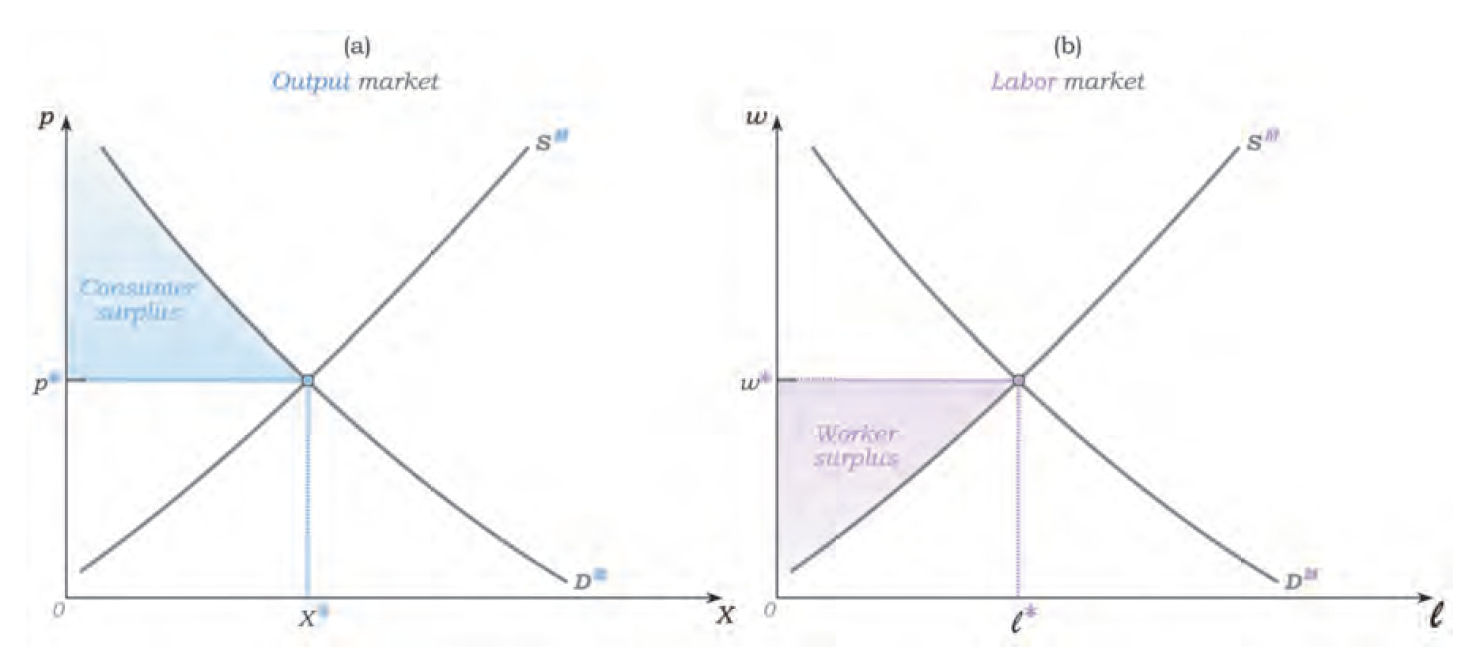
\includegraphics[width=1\textwidth]{15_1} %插入图片,[]中设置图片大小,{}中是图片文件名
	\caption{Aggregate Consumer and Worker Surplus when Tastes Are Quasilinear} %最终文档中希望显示的图片标题
	\label{Fig.main2} %用于文内引用的标签
\end{figure}


\subsection{“生产者剩余”或利润}
经济利润是生产者从参与市场活动所得到的“剩余”的度量。因为,我们将交替地使用生产者剩余(consumer surplus)和经济利润(economic profit)的术语。利润可以表示为生产者供给曲线上方的面积。

\begin{figure}[H] %H为当前位置,!htb为忽略美学标准,htbp为浮动图形
	\centering %图片居中^{}
	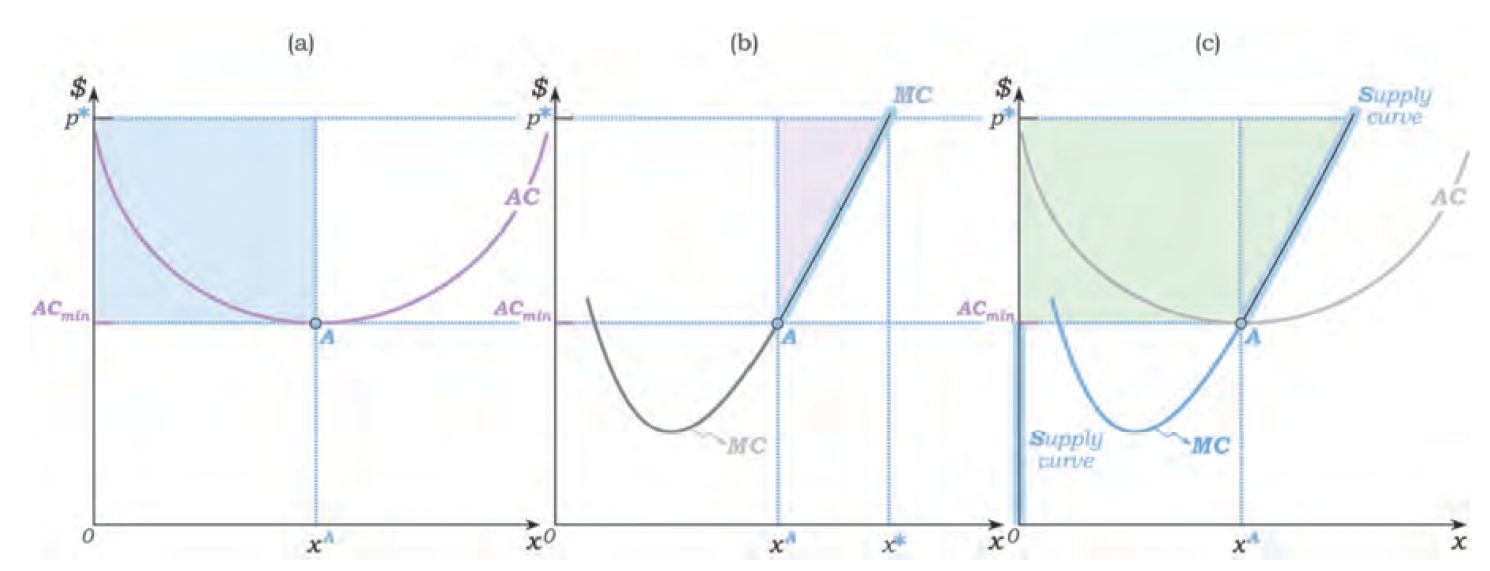
\includegraphics[width=1\textwidth]{15_2} %插入图片,[]中设置图片大小,{}中是图片文件名
	\caption{Three Ways of Illustrating Short-Run Profit or Short-Run Producer Surplus} %最终文档中希望显示的图片标题
	\label{Fig.main3} %用于文内引用的标签
\end{figure}

对生产者来说,在加总生产者并把他们看作单一的代表性消费者方面没有类似收入效应的困难。因而,当我们把个体生产者供给曲线加总成市场供给曲线时,市场供给曲线以上的面积为个体供给曲线以上面积的加总。也就是说可以把市场供给曲线看成单一代表性生产者的供给曲线。

劳动市场的生产者剩余

\begin{figure}[H] %H为当前位置,!htb为忽略美学标准,htbp为浮动图形
	\centering %图片居中^{}
	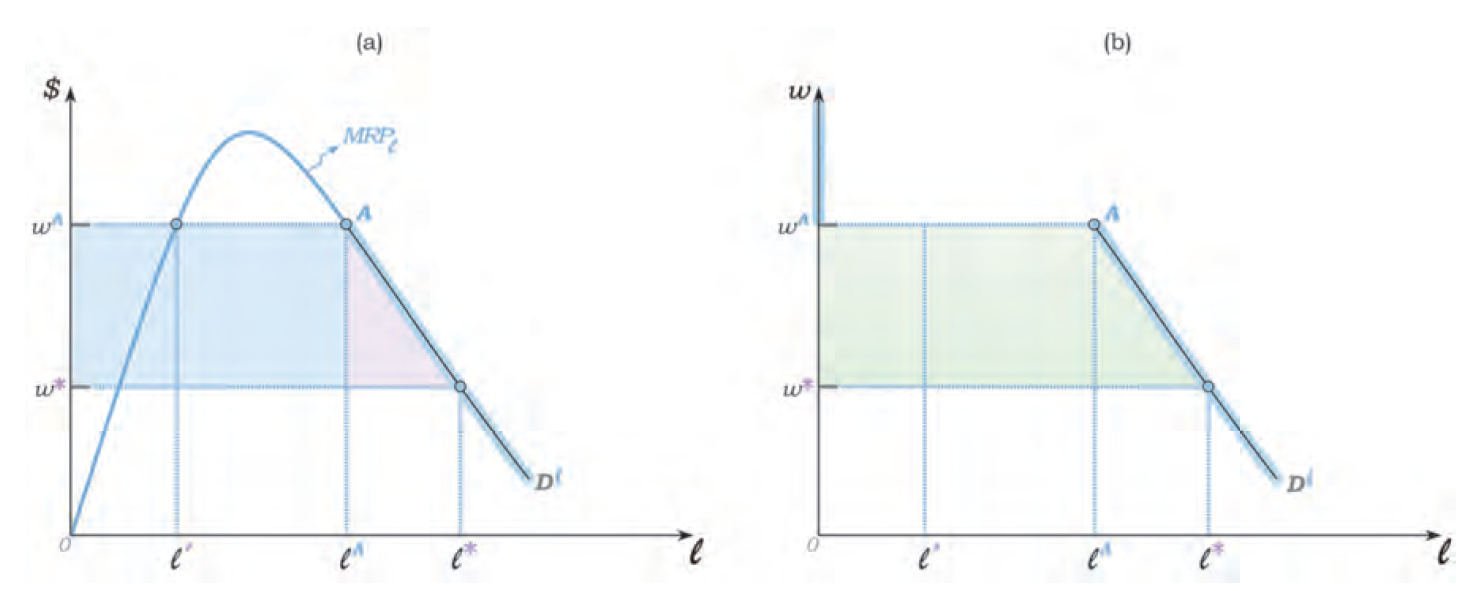
\includegraphics[width=1\textwidth]{15_3} %插入图片,[]中设置图片大小,{}中是图片文件名
	\caption{Producer Surplus in Labor Markets} %最终文档中希望显示的图片标题
	\label{Fig.main4} %用于文内引用的标签
\end{figure}

假定市场工资是$ w^* $并且企业在$ l^A $处停止雇佣。那么我们可以问企业,该情况与持平工资对应的零利润相比创造了多少额外利润。

\hspace*{\fill}

把所有剩余放在一起

\begin{figure}[H] %H为当前位置,!htb为忽略美学标准,htbp为浮动图形
	\centering %图片居中^{}
	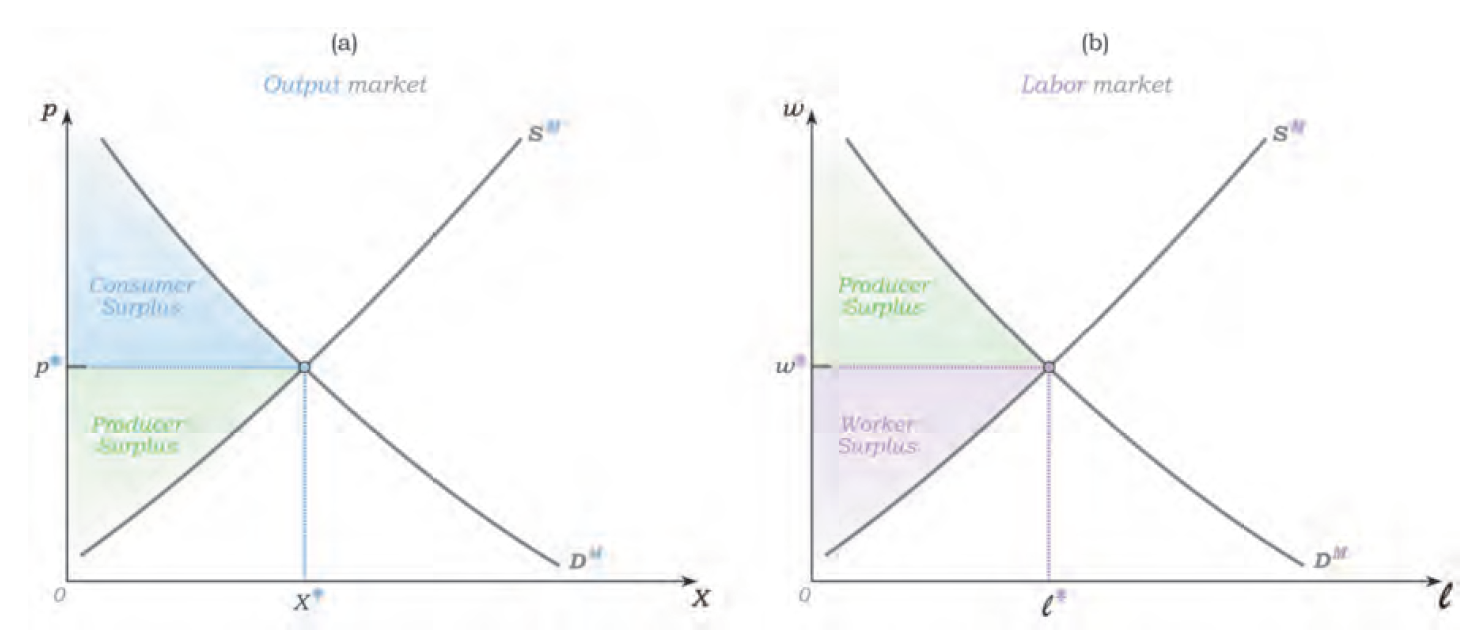
\includegraphics[width=1\textwidth]{15_4} %插入图片,[]中设置图片大小,{}中是图片文件名
	\caption{Surpluses in Output and Labor Markets} %最终文档中希望显示的图片标题
	\label{Fig.main5} %用于文内引用的标签
\end{figure}

\subsection{看不见的手与福利经济学第一定理}

画出边际社会收益MSB(marginal social benefit)与编辑社会成本MSC(marginal social cost)

\begin{figure}[H] %H为当前位置,!htb为忽略美学标准,htbp为浮动图形
	\centering %图片居中^{}
	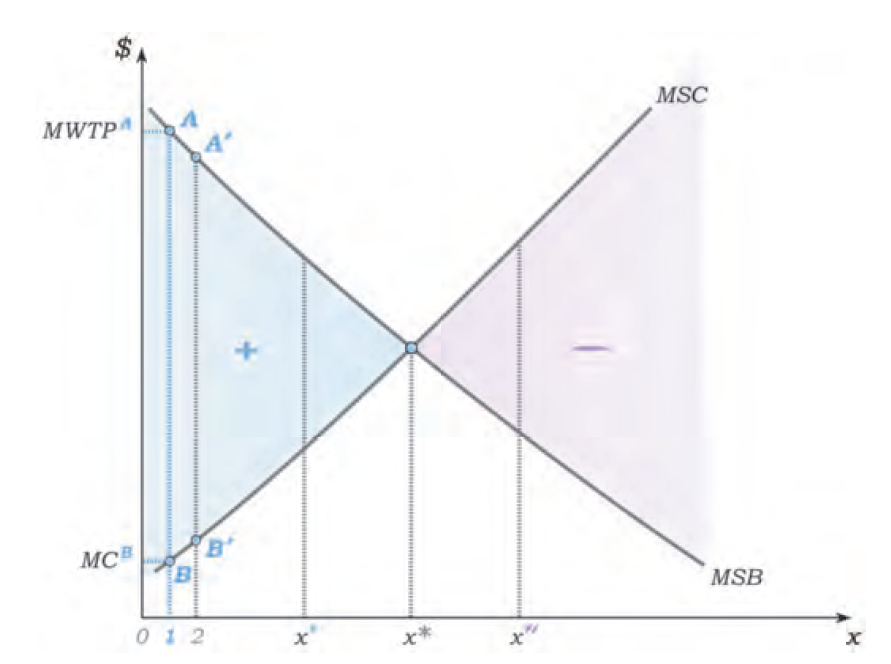
\includegraphics[width=1\textwidth]{15_5} %插入图片,[]中设置图片大小,{}中是图片文件名
	\caption{A Social Planner Finding the “Optimal” Output $ x^* $} %最终文档中希望显示的图片标题
	\label{Fig.main6} %用于文内引用的标签
\end{figure}

在给定消费者和生产者的处境的分散化市场情况下,他们仅自私地实现自身利益最大化所产生的市场需求和供给的交点,与上图中MSB和MSC曲线的交点完全相同。因此,如果社会规划者的目标是最大化社会总剩余,那么分散化市场生产的数量与社会规划者所选择的产量完全相同。

福利经济学第一定理指出,在一定条件下,市场是有效的。社会规划者能决定以不同于市场的方式分配社会剩余,与市场相比给予消费者会生产者更多,但总蛋糕的大小是不变的。

\hspace*{\fill}

包含在价格中的信息的关键作用

价格,不管是在投入市场还是在产出市场,都向消费者和生产者传递了他们所需要的信息,以使得他们“尽力做到最好”。

因为信息隐形地包含在价格中,所以个体在尽他们可能做到最好时,不需要知道他们个人处境以外的任何事情来确定他们下一步将做什么。市场中任何个体行动者不需要知道他的行为如何与更大的背景衔接起来,因为价格确保了我们二点行为相互融洽。这是分散化市场的一个巨大优势;市场不要求任何一个人拥有不易获得的信息。

自利的关键作用

分散化市场的第二个优势是有效市场均衡的产生不要求一个规划者的存在,相反,市场明确地依赖于个体,根据什么对他们来说是有利的感知来行动。

分散化市场产生了最大化社会剩余的结果,不仅是因为它们有效处理了信息,也因为它们依赖于掌控我们大多数行为的人性本质。

理性偏好假设并不是竞争性市场导致有效产出水平这个结果的必要条件。不假设个体的收入效应相互抵消,我们就不能把市场需求和总MWTP曲线堪称它们来自于一个单一的代表性消费者。但福利经济学第一定理的有效性并不取决于关于个体消费者偏好的假设。在偏好不是拟线性时,我们仅需要确定消费者剩余的精确大小时要谨慎,但是有效性结果仍成立。

但是,通过不允许市场需求被建模成一个代表性消费者的偏好的方式引进收入效应增加了一个重要的问题——虽则和分配方式的不同,偏好导致的有效产出水平不同。

\subsection{福利经济学第一定理背后的条件}

\subsubsection{价格的政策扭曲}

我们所做的第一个隐性假设是市场价格实际上如建模那样运行,它们被允许以向市场中众多的行动者发送无扭曲信号的方式形成。使这个信号变得扭曲的一个主要原因在于像税收、价格规制、工资控制、补贴项目,或在某些情形下一个市场显性的禁止等的可以的政府政策。

\subsubsection{外部性、社会成本与产权}

当外部性存在时,MSC和MSB的交点将与市场需求曲线和供给的交点不同。从而,在有外部性时,分散化市场不能生产有效的数量,市场价格以不能最大化社会剩余的方式发送给消费者和生产者去协调他们的行为。

\subsubsection{不对称信息}

除了外部性的缺失外,我们隐性假设了所有的经济人对市场的相关方面有相同的信息。

\subsubsection{市场势力}

假设经济中有市场势力(market power),也就是能影响经济环境本身的能力。当一个行业由单一企业或仅由几个企业组成时,每个企业将会足够大以至于影响行业中的经济环境,此时竞争性行为的假设被放松,福利经济学第一定理不一定成立。

\subsubsection{有效性VS其他社会目标}

有效并不一定是唯一目标,公平也很重要。

\section{均衡中的福利分析}

\subsection{消费者剩余}

只要个体偏好使得收入可以在个体消费者之间充分分配而没有总需求的变化,市场需求就具有个体需求曲线更一般的特性;即这样再分配所导致的需求变化相互之间完全抵消。

当收入变化时我们对商品$ x_i $的需求的变化必须与当我妻子的收入变化时需求的变化完全相同,不管初始时收入如何划分。
\[
\frac{\partial x_i^m}{\partial I^m}=\frac{\partial x_i^n}{\partial I^n}\enspace and\enspace \frac{\partial^2 x_i^m}{\partial (I^m)^2}=\frac{\partial^2 x_i^n}{\partial (I^n)^2}=0
\]

为了使从收入再分配的需求的变化相互抵消,需求关于收入的一阶导数必须相同;为使我们不管从哪里开始变化总是相互抵消,二阶导数必须为零。

需求函数一定采取如下形式:
\[
x^m_i(p_1,p_2,I^m)=a_i^m(p_1,p_2)+I^mb_i(p_1,p_2)
\]
\[
x^n_i(p_1,p_2,I^n)=a_i^n(p_1,p_2)+I^nb_i(p_1,p_2)
\]

其中$ a_i^m $表示关于商品i和个体m的函数,$ b_i $表示关于商品i但是对所有人都相同的函数。只要个体需求函数是这种形式(高曼形式),总需求函数就可以被当成产生于一个代表性消费者的效用最大化问题。

\hspace*{\fill}

总消费者剩余

\[
CS=\int_{p_1}^{\infty}h(p_1,p_2,u)dp
\]

当所有个体需求满足高曼形式时,可以把总市场需求当作产生于一个单一的代表性消费者。

\subsection{生产者剩余}

\[
Short-Run\enspace Producer\enspace Surplus=\int_{0}^{p}x_k^A(w,p)dp
\]
\[
Long-Run Producer Surplus=\int_{0}^{p}x(w,p)dp
\]

其中$ x_k^A $和$ x $是短期和长期供给函数。由于成本函数可以被加总,并由于市场攻击函数可以被理解为产生于单一的代表性企业总生产者剩余可以用上式衡量。

\subsection{福利经济学第一定理}

可以把社会规划者看作一个同时是代表性消费者和生产者并简单地试图最大化自身福利的人,他知道生产x的长期成本,这使得他能够花出社会可能性边界,也就是一个社会范围的约束,即我们根据符合商品y来生产更多的x时面临的权衡取舍。由于复合商品y的价格是单位价格,我们能生产最多的y等于社会中所有消费者的总收入I。

如果我们现在知道效用函数U(x,y)可以表示成“代表性消费者”的偏好,我们就可以把社会规划者试图最大化世界的社会剩余问题写成:

\[
\max\limits_{x,y}U(x,y)\enspace s.t. \enspace I=px+y
\]

	
\end{document}